 \begin{frame}[fragile]{Funktion random\_binom(n, p)}
  \begin{columns}
  \column{.49\textwidth}
    \begin{itemize}
  	\item Erzeugt binomialverteilte Zufallszahl
  	\item $ z := |\left\{ i|u_i<p \right\}|$
  \end{itemize}
  \begin{lstlisting}[language=python]
def random_binom(n, p):
    z = 0
    # create n random numbers
    # between [0,1]:
    for i in range(n):
        rand = random.random()
        z += 1 if rand < p else 0
    return z
\end{lstlisting}
\logopythonbottom
  \column{.49\textwidth}
    	\begin{figure}[h!]
    	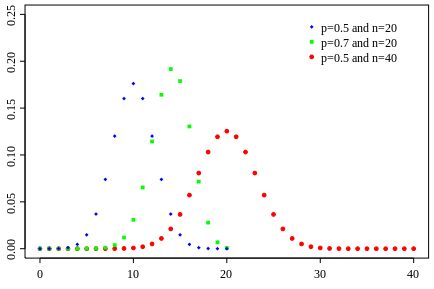
\includegraphics[scale=0.5]{lib_random_binom_wahrscheinlichkeitsverteilung.png}
  			\caption{Wahrscheinlichkeitsverteilung der Binomialverteilung \tiny{(Wikipedia)}}
		\end{figure}
  \end{columns}
\end{frame}	